\section{Data Pipeline Implementation}
\label{sec:4_3}

\subsection{ETL Pipeline}
\label{sec:4_3_1}

The ETL pipeline processes the two raw data sources into analysis-ready format using Polars for memory-efficient operations:

\begin{enumerate}
    \item \textbf{Insertion Lifecycle Events:} Listing data snapshots capturing status transitions and property attributes (804,717 events)
    \item \textbf{SEON Transaction Records:} Browser/device interaction data captured when users submit listings for approval ($\sim$140,000 transactions)
\end{enumerate}

The pipeline uses Polars lazy evaluation for streaming processing on commodity hardware. The critical \texttt{correlate\_events\_to\_seon} function matches each listing event to its corresponding SEON transaction the browser interaction data collected when that listing was submitted. The matching uses bidirectional as-of joins: (1) a forward join finds the nearest SEON record after the event timestamp, (2) a backward join finds the nearest SEON record before the event, and (3) the results are merged with preference for forward matches. This ensures each listing event is paired with its submission-time SEON signals (device fingerprint, IP intelligence, behavioral indicators) while handling edge cases where SEON data may be missing before or after specific events. Complete implementation is provided in Appendix~A.

\begin{figure}[htbp]
    \centering
    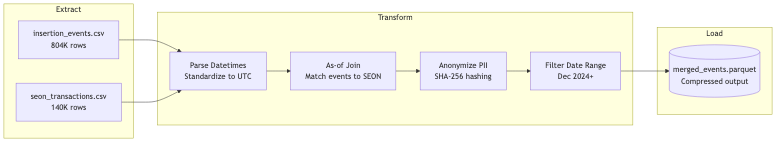
\includegraphics[width=\textwidth]{figures/fig_4_4_2_1.png}
    \caption{ETL Pipeline Flow: Extract → Transform → Load}
    \label{fig:4_2}
\end{figure}

\textbf{Datetime Standardization:} The two data sources use different timestamp formats requiring normalization:
\begin{itemize}
    \item \textbf{Insertion Lifecycle Events:} \texttt{\%Y-\%m-\%d \%H:\%M:\%S\%.\%f \%z} (space-separated timezone, e.g., ``2025-01-15 10:30:45.123 +0100'')
    \item \textbf{SEON Transactions:} \texttt{\%Y-\%m-\%dT\%H:\%M:\%S\%.\%f\%z} (ISO 8601 format, e.g., ``2025-01-15T10:30:45.123+0000'')
\end{itemize}

All timestamps are converted to UTC for consistent temporal operations across both sources.

\textbf{PII Anonymization:} Identity columns are hashed before any analysis using HMAC-SHA256 with type-specific salts. The implementation in \texttt{src/utils/anonymize.py} handles component-based anonymization for emails (user/domain), phones (country/area/number), IPs (network/host), and addresses.

Output Parquet files use Snappy compression, reducing storage by $\sim$70\% while maintaining fast read performance.

\subsection{Temporal Splitting}
\label{sec:4_3_2}

The \texttt{TemporalSplitter} class implements point-in-time label assignment to prevent label leakage. Only fraud flags occurring before the cutoff date are assigned as positive labels, ensuring temporal integrity of the training and test sets.
